

\begin{figure}[h]

\begin{subfigure}[b]{.5\linewidth}
\centering 
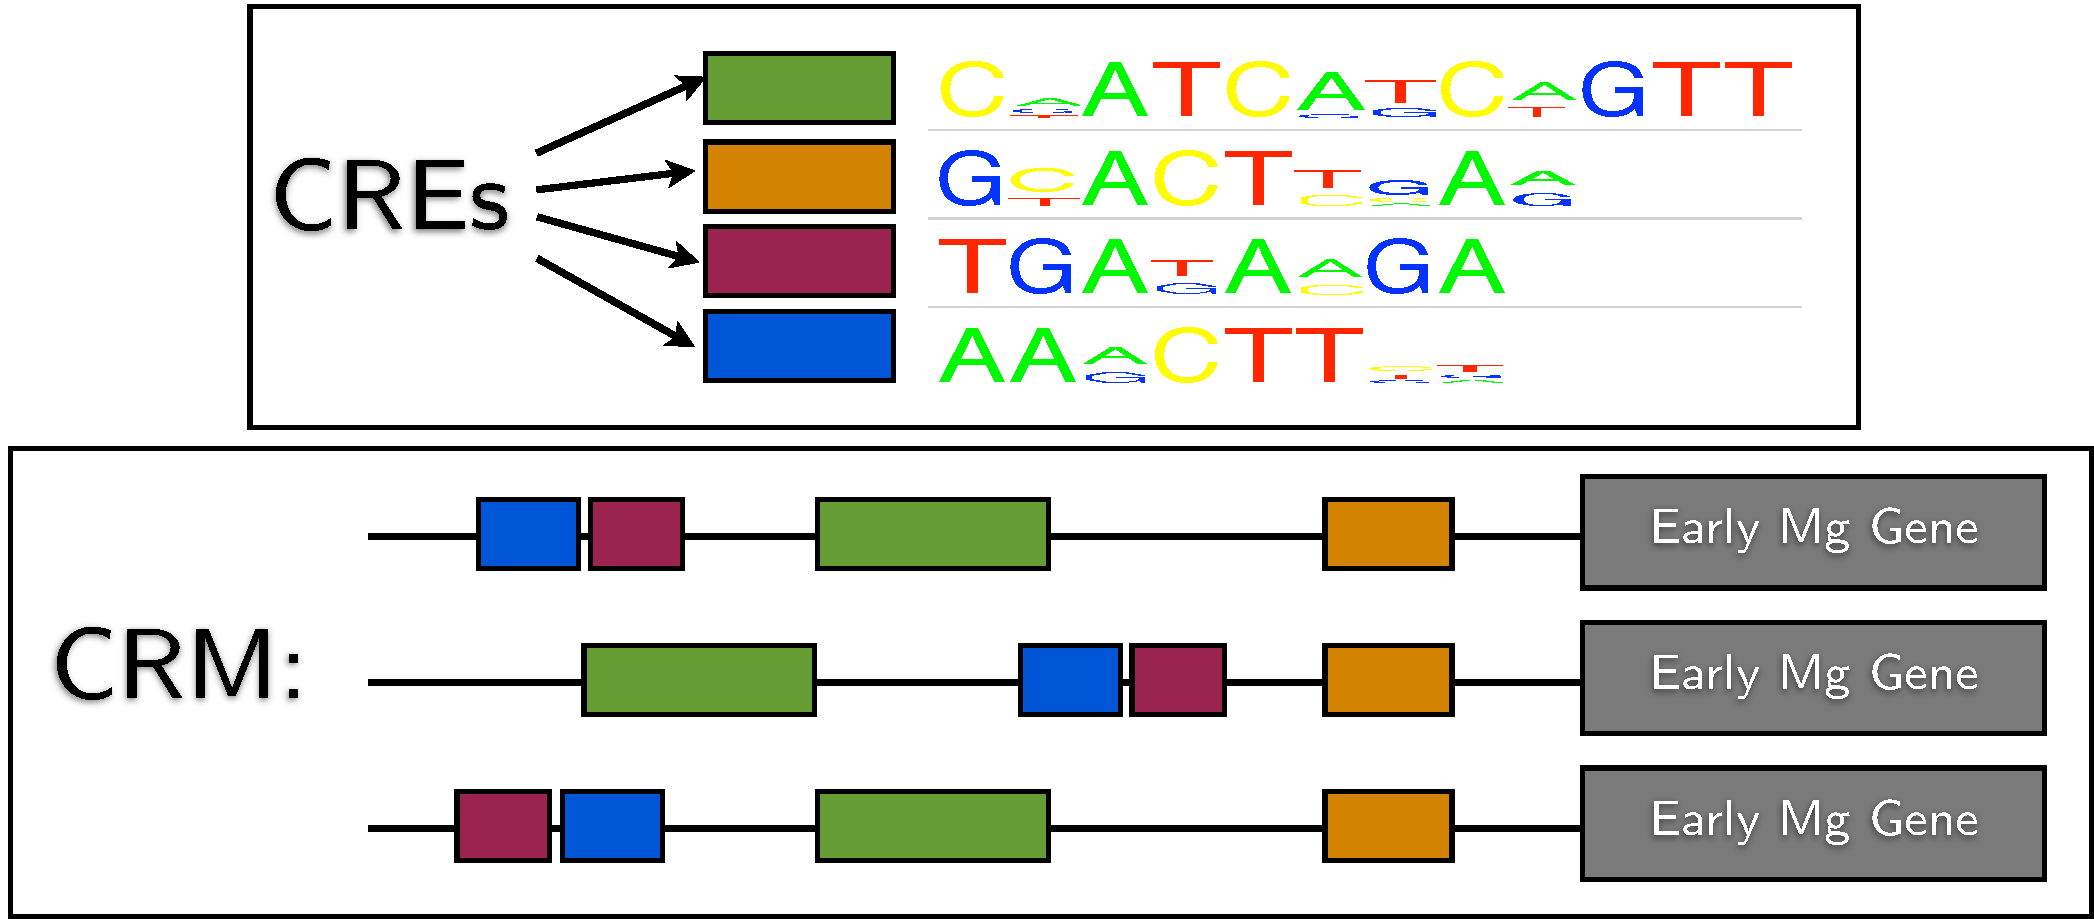
\includegraphics[width=0.9\linewidth]{figures/figs/CREvCRM.pdf}
\caption{}\label{fig:cre-crm-intro-a}
\end{subfigure}%
\hfil
\begin{subfigure}[b]{.5\linewidth}
\centering
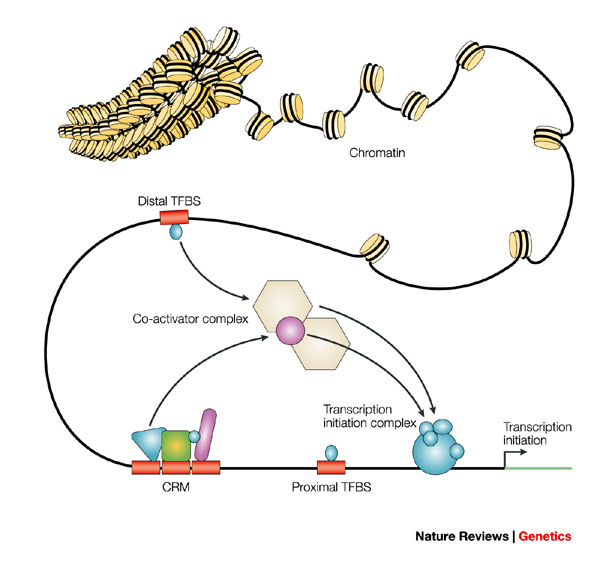
\includegraphics[width=0.9\linewidth]{figures/figs/elementsOfTxReg.jpeg}
\caption{}\label{fig:cre-crm-intro-b}
\end{subfigure}

\caption[Elements of transcriptional regulation]{\sf \textbf{Elements of transcriptional regulation} \\
(A) The relationship between \glspl{CRE} (colored rectangles) and \glspl{CRM}: the colored rectangles represent position specific scoring matrix information (top) that defines an individual \gls{CRE}.
(B) \glspl{TF} bind to specific sites (\glspl{TFBS}) that are either proximal or distal to a transcription start site. Sets of \glspl{TF} can operate in functional \glspl{CRM} to achieve specific regulatory properties. Interactions between bound \glspl{TF} and cofactors stabilize the transcription-initiation machinery to enable gene expression. The regulation that is conferred by sequence-specific binding \glspl{TF} is highly dependent on the three-dimensional structure of chromatin.\\

Panel B and corresponding legend text adapted from \citet{Wasserman2004}.
}\label{fig:cre-crm-intro}
\end{figure}